\documentclass[12pt]{article}

\usepackage[english]{babel}
\usepackage[utf8]{inputenc}
\usepackage{sansmathfonts}
\usepackage[T1]{fontenc}
\renewcommand*\familydefault{\sfdefault} %% Only if the base font of the document is to be sans serif
\usepackage{multicol,lipsum}
\usepackage{amsmath,cancel}
\usepackage{amssymb,amsthm,dsfont,mathrsfs}
\usepackage[colorinlistoftodos]{todonotes}
\usepackage{geometry}
\geometry{
a4paper,
total={170mm,257mm},
left=20mm,
top=15mm,
bottom=22mm,
}
\usepackage{natbib}
\usepackage{soul}
\usepackage{setspace}
\usepackage{hyperref}
\usepackage{xcolor}
\usepackage{graphicx}
\usepackage{tikz}
\usepackage{siunitx}
\graphicspath{ {imagens/} }
\usepackage{fancyhdr}
\pagestyle{fancy}
\renewcommand{\headrulewidth}{0pt}

\color{darkgray}
\newcommand{\T}[1]{\vspace{0.4cm}\textbf{\large#1}}
\newcommand{\TW}[1]{\textbf{\large#1}}

\newcommand{\TM}[1]{\vspace{0.2cm} \textbf{#1}}

\newcommand{\M}[1]{
\vspace{-0.6cm}
\begin{flalign*}
#1&
\end{flalign*}
\vspace{-0.6cm}
}


\definecolor{bluebell}{rgb}{0.25, 0.35, 0.89} 
\definecolor{laranja}{rgb}{0.87, 0.48, 0.25} 
\definecolor{verde}{rgb}{0, 0.54, 0.44} 
\definecolor{babypink}{rgb}{1, 0.42, 0.52} 
\definecolor{rosa}{rgb}{1, 0.72, 0.77} 
\definecolor{cinza}{rgb}{0.3, 0.3, 0.3}  
\definecolor{iris}{rgb}{0.25, 0.35, 0.89}  
\definecolor{babyblue}{rgb}{0.13, 0.59, 0.95}

\setlength\columnsep{30pt}

\setlength{\parindent}{0cm}
\setlength{\fboxrule}{1.3pt}  % <-- Aumenta a espessura

\newcommand{\Formula}[1]{
\begin{center}
\color{iris}
\fcolorbox{rosa}{white}{
\(
\begin{array}{c}
#1
\end{array}
\)
}
\color{cinza}
\end{center}
}

\begin{document}
\pagenumbering{gobble}
\setstretch{1.3}


\includegraphics[width=4cm]{Logo2.png}
\begin{center}
    \textbf{\Huge \textcolor{bluebell}{Lei dos Senos e Cossenos}}
\end{center}

\begin{multicols}{2}

\vspace{0.4cm}
\TW{Descrição} 

As leis dos senos e dos cossenos são fundamentais na trigonometria para resolver triângulos, especialmente os não retângulos, permitindo calcular lados e ângulos quando o Teorema de Pitágoras não pode ser utilizado.

\vspace{0.4cm}
\TW{Lei dos Senos}

A Lei dos Senos relaciona os comprimentos dos lados de um triângulo com os senos de seus ângulos opostos. Em qualquer triângulo \(ABC\), com lados \(a\), \(b\), e \(c\) opostos aos ângulos \(A\), \(B\) e \(C\), a Lei dos Senos é expressa por:

\Formula{
\dfrac{a}{sen~ A} = \dfrac{b}{sen~ B} = \dfrac{c}{sen~ C}
}

\vspace{-0.2cm}
\TM{Exemplo:}

\begin{center}
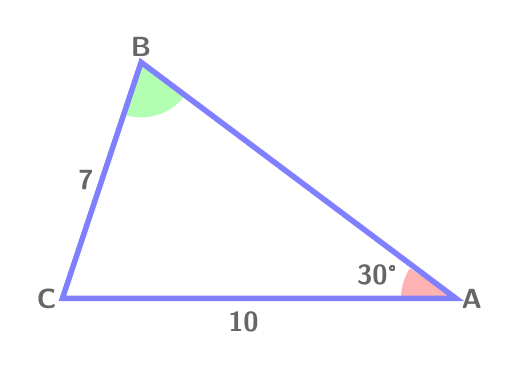
\begin{tikzpicture}
\tikzstyle{texto}=[draw=none,fill=none,black!60!white]
\tikzstyle{line}=[blue!50!white,line width=2pt]
\tikzstyle{angleA}=[draw=none,fill=red!30!white]
\tikzstyle{angleB}=[draw=none,fill=green!30!white]

\begin{scope}[shift={(5,0)}]
    \draw[angleA] (0,0) -- (147:0.7) arc (147:180:0.7);
\end{scope}
\begin{scope}[shift={(1,3)}]
    \draw[angleB] (0,0) -- (250:0.7) arc (250:320:0.7);
\end{scope}
\draw[line] (0,0) -- (5,0) -- (1,3) -- cycle;

\node[texto] at (4,0.3) {\textbf{\textbf{30°}}};
\node[texto] at (5.2,0) {\textbf{\textbf{A}}};
\node[texto] at (1,3.2) {\textbf{\textbf{B}}};
\node[texto] at (-0.2,0) {\textbf{\textbf{C}}};
\node[texto] at (0.3,1.5) {\textbf{7}};
\node[texto] at (2.3,-0.3) {\textbf{10}};
\end{tikzpicture}
\end{center}
\vspace{-0.3cm}
Nesse triângulo temos, \(a=7\), \(b=10\) e \(A = 30^\circ\).
Para encontrar o ângulo \(B\) temos:

\[
\dfrac{7}{sen~ 30^\circ} = \dfrac{10}{sen~ B}
\]

\M{7 \cdot sen~ B &= 10 \cdot sen~ 30^\circ = 10 \cdot \dfrac{1}{2}}
\M{7 \cdot sen~ B &= 5}
\M{sen~ B &= \dfrac{5}{7} \approx 0.7143}
\M{B &\approx sen~^{-1}(0.7143) \approx 45.57^\circ}

\TW{Lei dos Cossenos}

A Lei dos Cossenos é usada para calcular um lado de um triângulo quando os outros dois lados e o ângulo entre eles são conhecidos, ou para determinar um ângulo quando todos os lados do triângulo são conhecidos.
Em um triângulo \(ABC\), a Lei dos Cossenos é expressa por:

\Formula{
a^2 = b^2 + c^2 - 2bc \cdot \cos A
}

\vspace{-0.2cm}
\TM{Exemplo:}
\vspace{-0.3cm}
\begin{center}
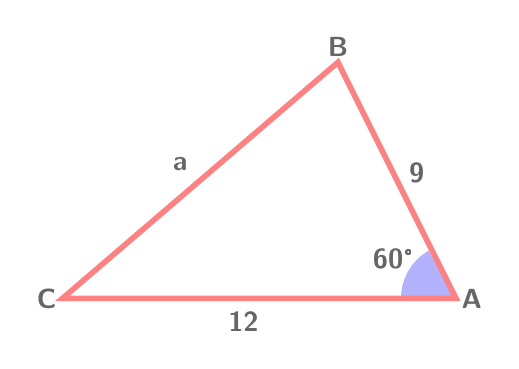
\begin{tikzpicture}
\tikzstyle{texto}=[draw=none,fill=none,black!60!white]
\tikzstyle{line}=[red!50!white,line width=2pt]
\tikzstyle{angleA}=[draw=none,fill=blue!30!white]

\begin{scope}[shift={(5,0)}]
    \draw[angleA] (0,0) -- (120:0.7) arc (120:180:0.7);
\end{scope}

\draw[line] (0,0) -- (5,0) -- (3.5,3) -- cycle;

\node[texto] at (4.2,0.5) {\textbf{\textbf{60°}}};
\node[texto] at (5.2,0) {\textbf{\textbf{A}}};
\node[texto] at (3.5,3.2) {\textbf{\textbf{B}}};
\node[texto] at (-0.2,0) {\textbf{\textbf{C}}};
\node[texto] at (1.5,1.7) {\textbf{a}};
\node[texto] at (2.3,-0.3) {\textbf{12}};
\node[texto] at (4.5,1.6) {\textbf{9}};
\end{tikzpicture}
\end{center}
\vspace{-0.3cm}
Nesse triângulo temos, \(b = 12\), \(c = 9\) e \(A = 60^\circ\). Sabemos que \(\cos~60^\circ = \frac{1}{2}\).

Para encontrar o valor de \(a\) temos:

\M{a^2 &= 12^2 + 9^2 - 2 \cdot 12 \cdot 9 \cdot \cos~60^\circ}
\M{a^2 &= 144 + 81 - 216 \cdot \dfrac{1}{2}}
\M{a^2 &= 225 - 108 = 117}
\M{a &= \sqrt{117}\approx 10,81}

\end{multicols}
\lfoot{\scriptsize © Copyright, Pratique Já}
\cfoot{\large \textcolor{bluebell}{pratiqueja.com}}
\end{document}